% !TeX root = ../build/main.tex

When a new voting process begins, the Sequencer initializes a new State, represented by the root hash of a Merkle tree. This tree encapsulates all essential information about the voting process, including process parameters, voter registry (census), ballot configurations, and initial results.

For each new batch of votes, the Sequencer updates the state by generating a zkSNARK proof that \textbf{validates the state transition from the current Root to a new Root}. This proof is submitted on-chain for settlement. By doing so, we maintain an immutable and verifiable record of the voting process on the blockchain.

This approach allows anyone to access the latest verified state of the voting process from the Results Verification smart contract, along with the necessary data to process subsequent state updates. The system's design enables multiple Sequencers to participate in tallying votes. They can take the current State Root and its associated data to construct the next state, incorporating new votes into the tally. This decentralization of Sequencers helps prevent potential censorship and reinforces the robustness of the voting process.

\subsection{Maintaining the Chain}

The chain of integrity is maintained through a combination of smart contract enforcement and strict zkSNARK circuit constraints. This ensures that each state transition is valid and builds upon the last accepted state without requiring additional mechanisms.

\begin{itemize}
	\item \textbf{Sequential State Roots}: Each state transition updates the Merkle tree from a previous root (`Root1`) to a new root (`Root2`) after processing a batch of votes.
	\item \textbf{Smart Contract Enforcement}: The smart contract verifies that the `Root1` provided in the zkSNARK proof matches the last committed state root stored on-chain. This guarantees that all transitions are sequential and based on the latest accepted state.
	\item \textbf{Proof Validation}: The smart contract uses the zkSNARK verification key to validate the submitted proof. A valid proof confirms that the transition from `Root1` to `Root2` adheres to all protocol rules enforced by the circuit.
	\item \textbf{State Update}: Upon successful verification, the smart contract updates the stored state root hash to`Root2`, ensuring an immutable and continuous chain of states.
\end{itemize}

\subsection{State Merkle Tree Structure}

The State tree contains some special addresses (indices) for storing some required data regarding the voting process:

\begin{itemize}
	\item Address `0x0`: \textbf{Process Identifier}: stores a unique identifier for the voting process.
	\item Address `0x1`: \textbf{Census Root and Type}: contains the information necessary to validate vote proofs.
	\item Address `0x2`: \textbf{Ballot Mode}: encodes rules for validating votes, such as the maximum number of selectable options.
	\item Address `0x3`: \textbf{Threshold Encryption key}: the public key used to encrypt the votes.
	\item Address `0x4`: \textbf{Added Results Accumulator}: stores the aggregated encrypted voting results that need to be added.
	\item Address `0x5`: \textbf{Subtract Results Accumulator}: stores the aggregated encrypted voting results that need to be subtracted.
	\item Any Address: \textbf{Vote addresses}: are stored within the State tree pointing to a voter's identity commitment. Each commitment is a 32-byte hash derived from the voter's unique information and a secret.
	\item Any Address: \textbf{Vote nullifiers}: are stored within the State tree to prevent double voting and to allow vote overwrite. Each nullifier is a 32-byte hash derived from the voter's commitment and a secret.
\end{itemize}

\begin{figure}[H]
	\centering
	\fbox{
		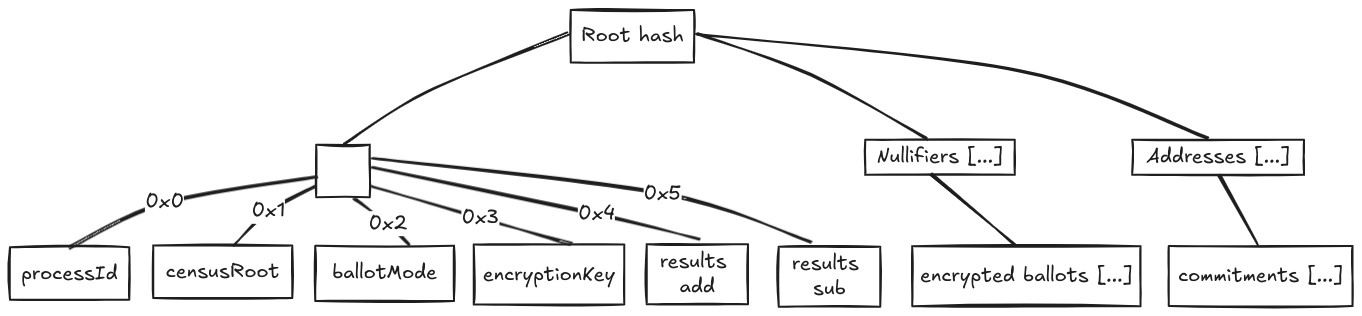
\includegraphics[scale = 0.3, draft = false]{\figs/merkle-tree-state.png}}
\end{figure}

\subsection{The Initial State}

The voting process begins with an initial state where the Merkle Tree Root is established and published on the Process Management smart contract. Predefined parameters are included, but the results are initialized to zero, and no nullifiers are present.

The Process Organizer transaction, contains the initial root and the necessary Merkle proofs. These proofs verify that the initial parameters are correct according to the voting process information and that no additional information is stored. Since the `ProcessId` of the initial state is a unique identifier, there won't be duplicate roots for different processes.

\subsection{State Transition}

To validate and process state transitions, \textbf{we employ a zkSNARK circuit that enforces all protocol constraints}. This circuit proves that the transition from the previous state Root to the new state Root is valid based on the newly processed votes.

\begin{figure}[H]
	\centering
	\fbox{
		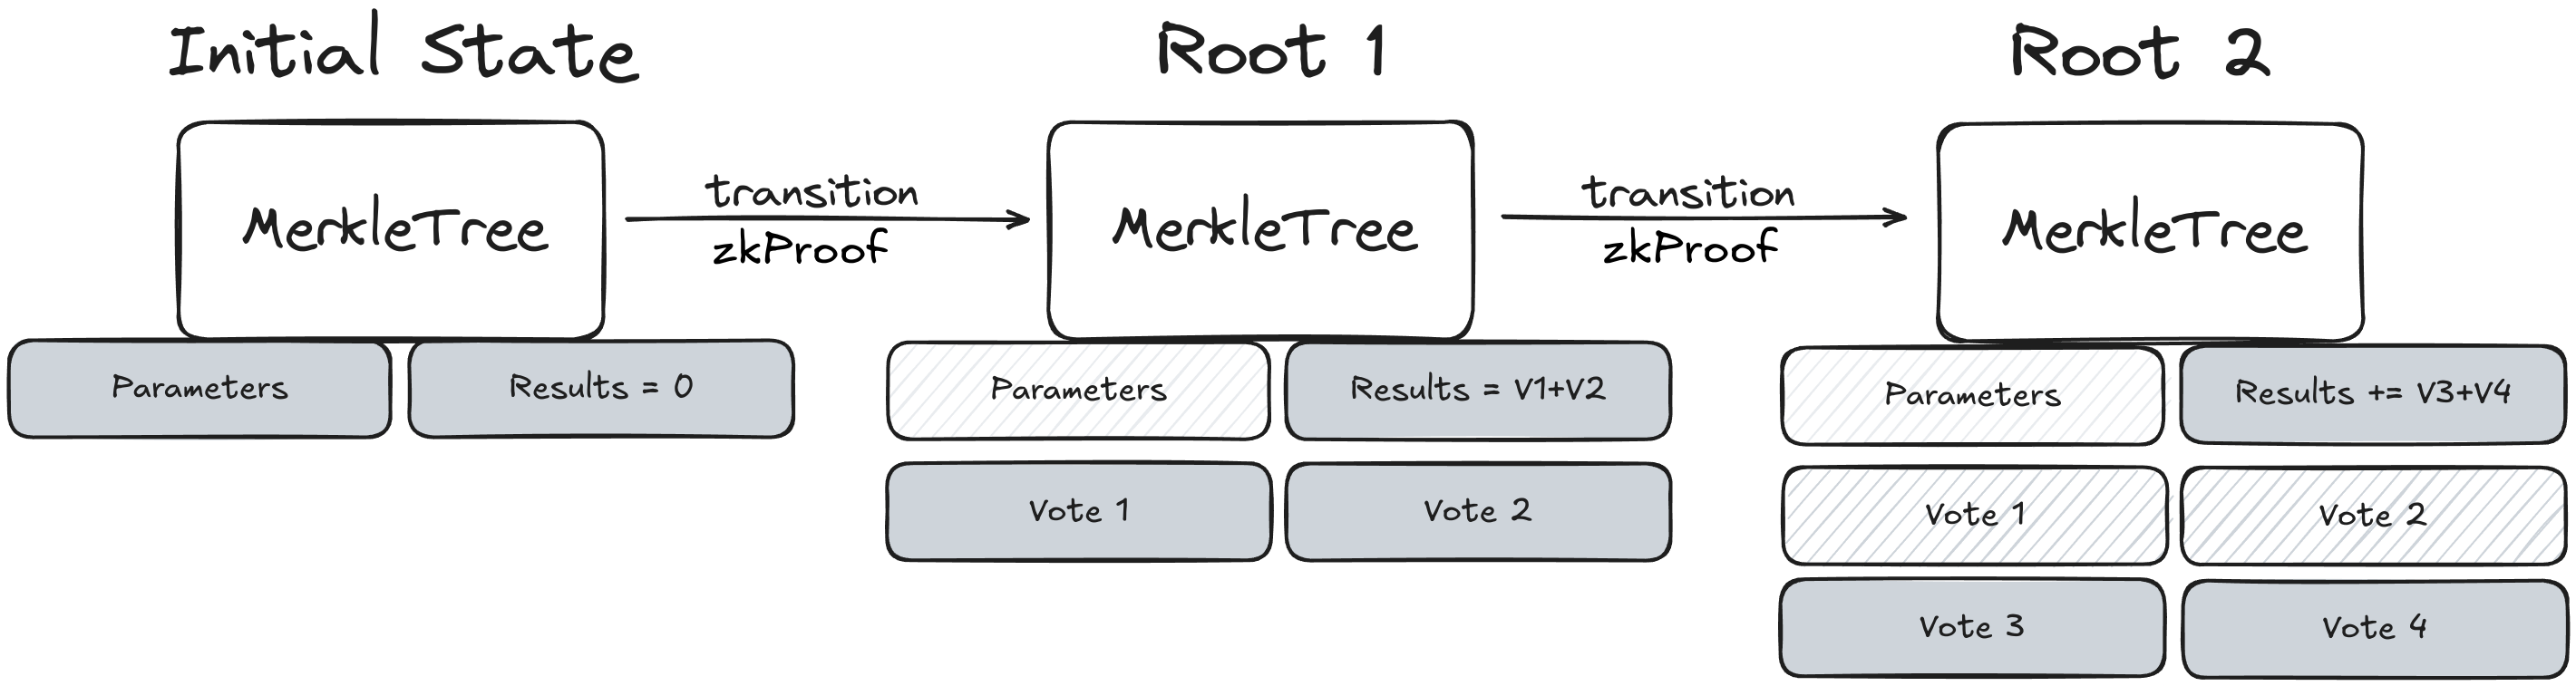
\includegraphics[scale = 0.12, draft = false]{\figs/state-transition.png}}
\end{figure}

The circuit have the following inputs (the public ones are required to verify the proof).

\begin{itemize}
	\item \textbf{Public Inputs:}
			\begin{itemize}
				\item Previous State Root (Root1): The Merkle tree root before the state transition.
				\item New State Root (Root2): The Merkle tree root after the state transition.
				\item Blob Data Commitment (blobCommitment): The commitment to the data blob containing the new votes.
			\end{itemize}
	\item \textbf{Private Inputs:}	
			\begin{itemize}
				\item Votes: The list of new votes being processed, including census proofs and authentication data.
				\item Merkle Proofs of nullifier inclusion: Proofs that each voter nullifier is included in the census.
				\item Merkle Proofs of results update: Proofs that the process results have been correctly updated.
				\item Merkle Tree Update Witnesses: Necessary data (e.g., Merkle paths) to update the Merkle tree from Root1 to Root2.
				\item Process Parameters: Retrieved from Root1 within the circuit.
			\end{itemize}
\end{itemize}

\begin{figure}[H]
	\centering
	\fbox{
		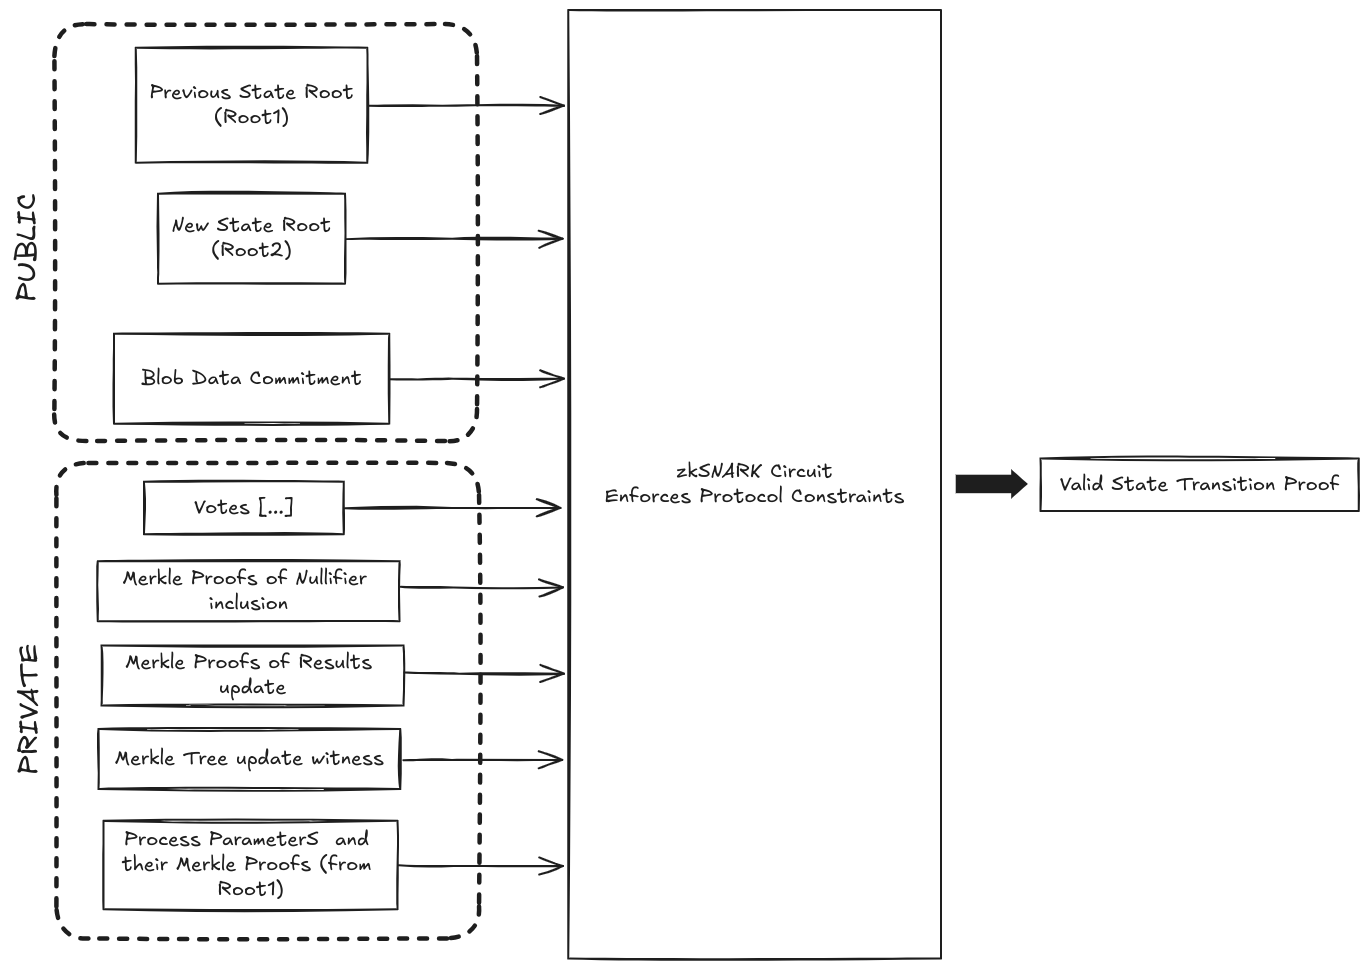
\includegraphics[scale = 0.3, draft = false]{\figs/circuit-inputs.png}}
\end{figure}

The following constraints must be enforced by the circuit.

\begin{itemize}
	\item \textbf{Immutable Process Parameters}: Ensure that critical process parameters (such as `censusRoot` or `processId`) retrieved from `Root1` remain consistent and are not altered in the transition.
	\item \textbf{Vote Validity}: Validate that each vote proof is correct.
	\item \textbf{Voter Eligibility}: Confirm that each voter is included in the census by verifying Merkle proofs of inclusion against the `censusRoot` retrieved from `Root1`.
	\item \textbf{Nullifier Non-Existence}: Ensure that the nullifier for each vote does not exist in the current state (`Root1`), preventing double voting.
	\item \textbf{Nullifier Addition}: Correctly add each new nullifier to the state, resulting in `Root2`, updating the Merkle tree accordingly.
	\item \textbf{Results Update}: Ensure that the voting results are accurately updated by adding the new votes to the previous results retrieved from `Root1`, so that `results2 = results1 + votes`.
	\item \textbf{Blob Data Integrity}: Confirm that the data used in the circuit (votes, nullifiers) corresponds to the `blobCommitment` provided as a public input, ensuring that the votes processed are exactly those published in the data blob.
	\item \textbf{State Transition Validity}: Ensure that the new state root (`Root2`) is correctly computed from `Root1` by applying the validated votes and updates to the Merkle tree.
\end{itemize}

\subsection{Finalization of the Voting Process}

At the conclusion of the voting period, the smart contract ceases to accept new state updates, effectively finalizing the process. The final State is then available on-chain for verification, providing an immutable record of the voting outcome.